\documentclass[final]{beamer}
\usepackage[orientation=landscape, size=custom, width=100cm, height=70cm, scale=1.4]{beamerposter}

\usepackage[swedish]{babel}
\usepackage[T1]{fontenc}
\usepackage[utf8]{inputenc}

\usepackage{lmodern}
\usepackage{hyphenat}
\usepackage{microtype}
\usepackage{parskip}
\usepackage{float}
\usepackage{graphicx}
\usepackage{booktabs}

\usebackgroundtemplate{
\includegraphics[width=\paperwidth]{figures/header.pdf}}

% https://www.komm.umu.se/grafisk-profil/
\definecolor{umublue}{RGB}{0,61,165}
\definecolor{umulightblue}{RGB}{0,160,230}
\definecolor{umugreen}{RGB}{80,190,31}

\setbeamercolor{titlelike}{fg=white}
\setbeamercolor{author}{fg=white}
\setbeamercolor{institute}{fg=white}
\setbeamercolor{block title}{fg=umublue,bg=white}
\setbeamercolor{block body}{fg=black,bg=white}
\setbeamercolor{block alerted title}{fg=white,bg=umublue}
\setbeamercolor{block alerted body}{fg=black,bg=dblue!10}

\newlength{\onecolwid}
\setlength{\onecolwid}{0.2\textwidth} % Width of one column

\title{Ytgående farkost för vattenrening}
\author{Anton Eriksson, Emelie Nordlinder, Jenny Bergman,
  Jesper Vesterberg, Joel Vedin, Johan Olofsson, Rasmus Nyman}
\institute{Design-Build-Test Grupp 5, Umeå Universitet}

\usepackage{atbegshi}% http://ctan.org/pkg/atbegshi
\AtBeginDocument{\AtBeginShipoutNext{\AtBeginShipoutDiscard}}

\begin{document}

\addtobeamertemplate{block end}{}{\vspace*{2ex}} % White space under blocks
\addtobeamertemplate{block alerted end}{}{\vspace*{2ex}} % White space under highlighted (alert) blocks

\setlength{\belowcaptionskip}{2ex} % White space under figures
\setlength\belowdisplayshortskip{2ex} % White space under equations

\begin{frame}[t]

  \begin{columns}[c]
    \begin{column}{\textwidth}
      \centering
      \vskip 1cm
      \usebeamercolor{title in headline}{\color{white}\Huge{\textbf{\inserttitle}}\\[0.5ex]}
      \usebeamercolor{author in headline}{\color{white}\insertauthor\\[0.8ex]}
      \usebeamercolor{institute in headline}{\color{white}\insertinstitute\\[1ex]}
      \vskip 2cm
    \end{column}
  \end{columns}

  \vspace{2cm}

  \begin{columns}[t, totalwidth=\textwidth]

    \begin{column}{0.0001\textwidth}\end{column} % Dummy column

    \begin{column}{\onecolwid}

      \begin{block}{Introduktion}

        SpinChem har utvecklat en \emph{roterande bäddreaktor}, RBR,
        som kan användas för att rena vattenmassor.

        Uppdraget var att utveckla
        en ytgående farkost som kan förflytta och driva dessa i t.ex. en sjö.
        På detta sätt kan föroreningar, t.ex. tungmetaller, plockas upp.

        Frågeställning: Hur effektivt kan farkosten rena en vattenmassa?

      \end{block}

      \begin{block}{Rening}
        Potentiella reningsmaterial att använda i RBRer har undersökts genom att
        utvärdera materialens kapacitet att ta upp metaller. Simuleringstester
        med flotten är gjorda i en bassäng innehållande basiskt vatten och en
        färgindikator som simulerar en förorening.

        I dessa simuleringstester
        laddades bäddreaktorerna med jonbytare.

      \end{block}

    \end{column}

    \begin{column}{\onecolwid}

      \begin{block}{Design}
        Farkosten designades med en modulär uppbyggnad:
          \begin{itemize}
          \item Utbytbara RBR-moduler med drivning och vågbrytare
          \item Kan användas med en eller två moduler
          \item Demonterbara pontoner, anpassningsbar flytkraft och lättare transport.
          \end{itemize}

        \vskip 5cm
        \begin{figure}[H]
          \centering
          \hbox{\hspace{-4.5cm}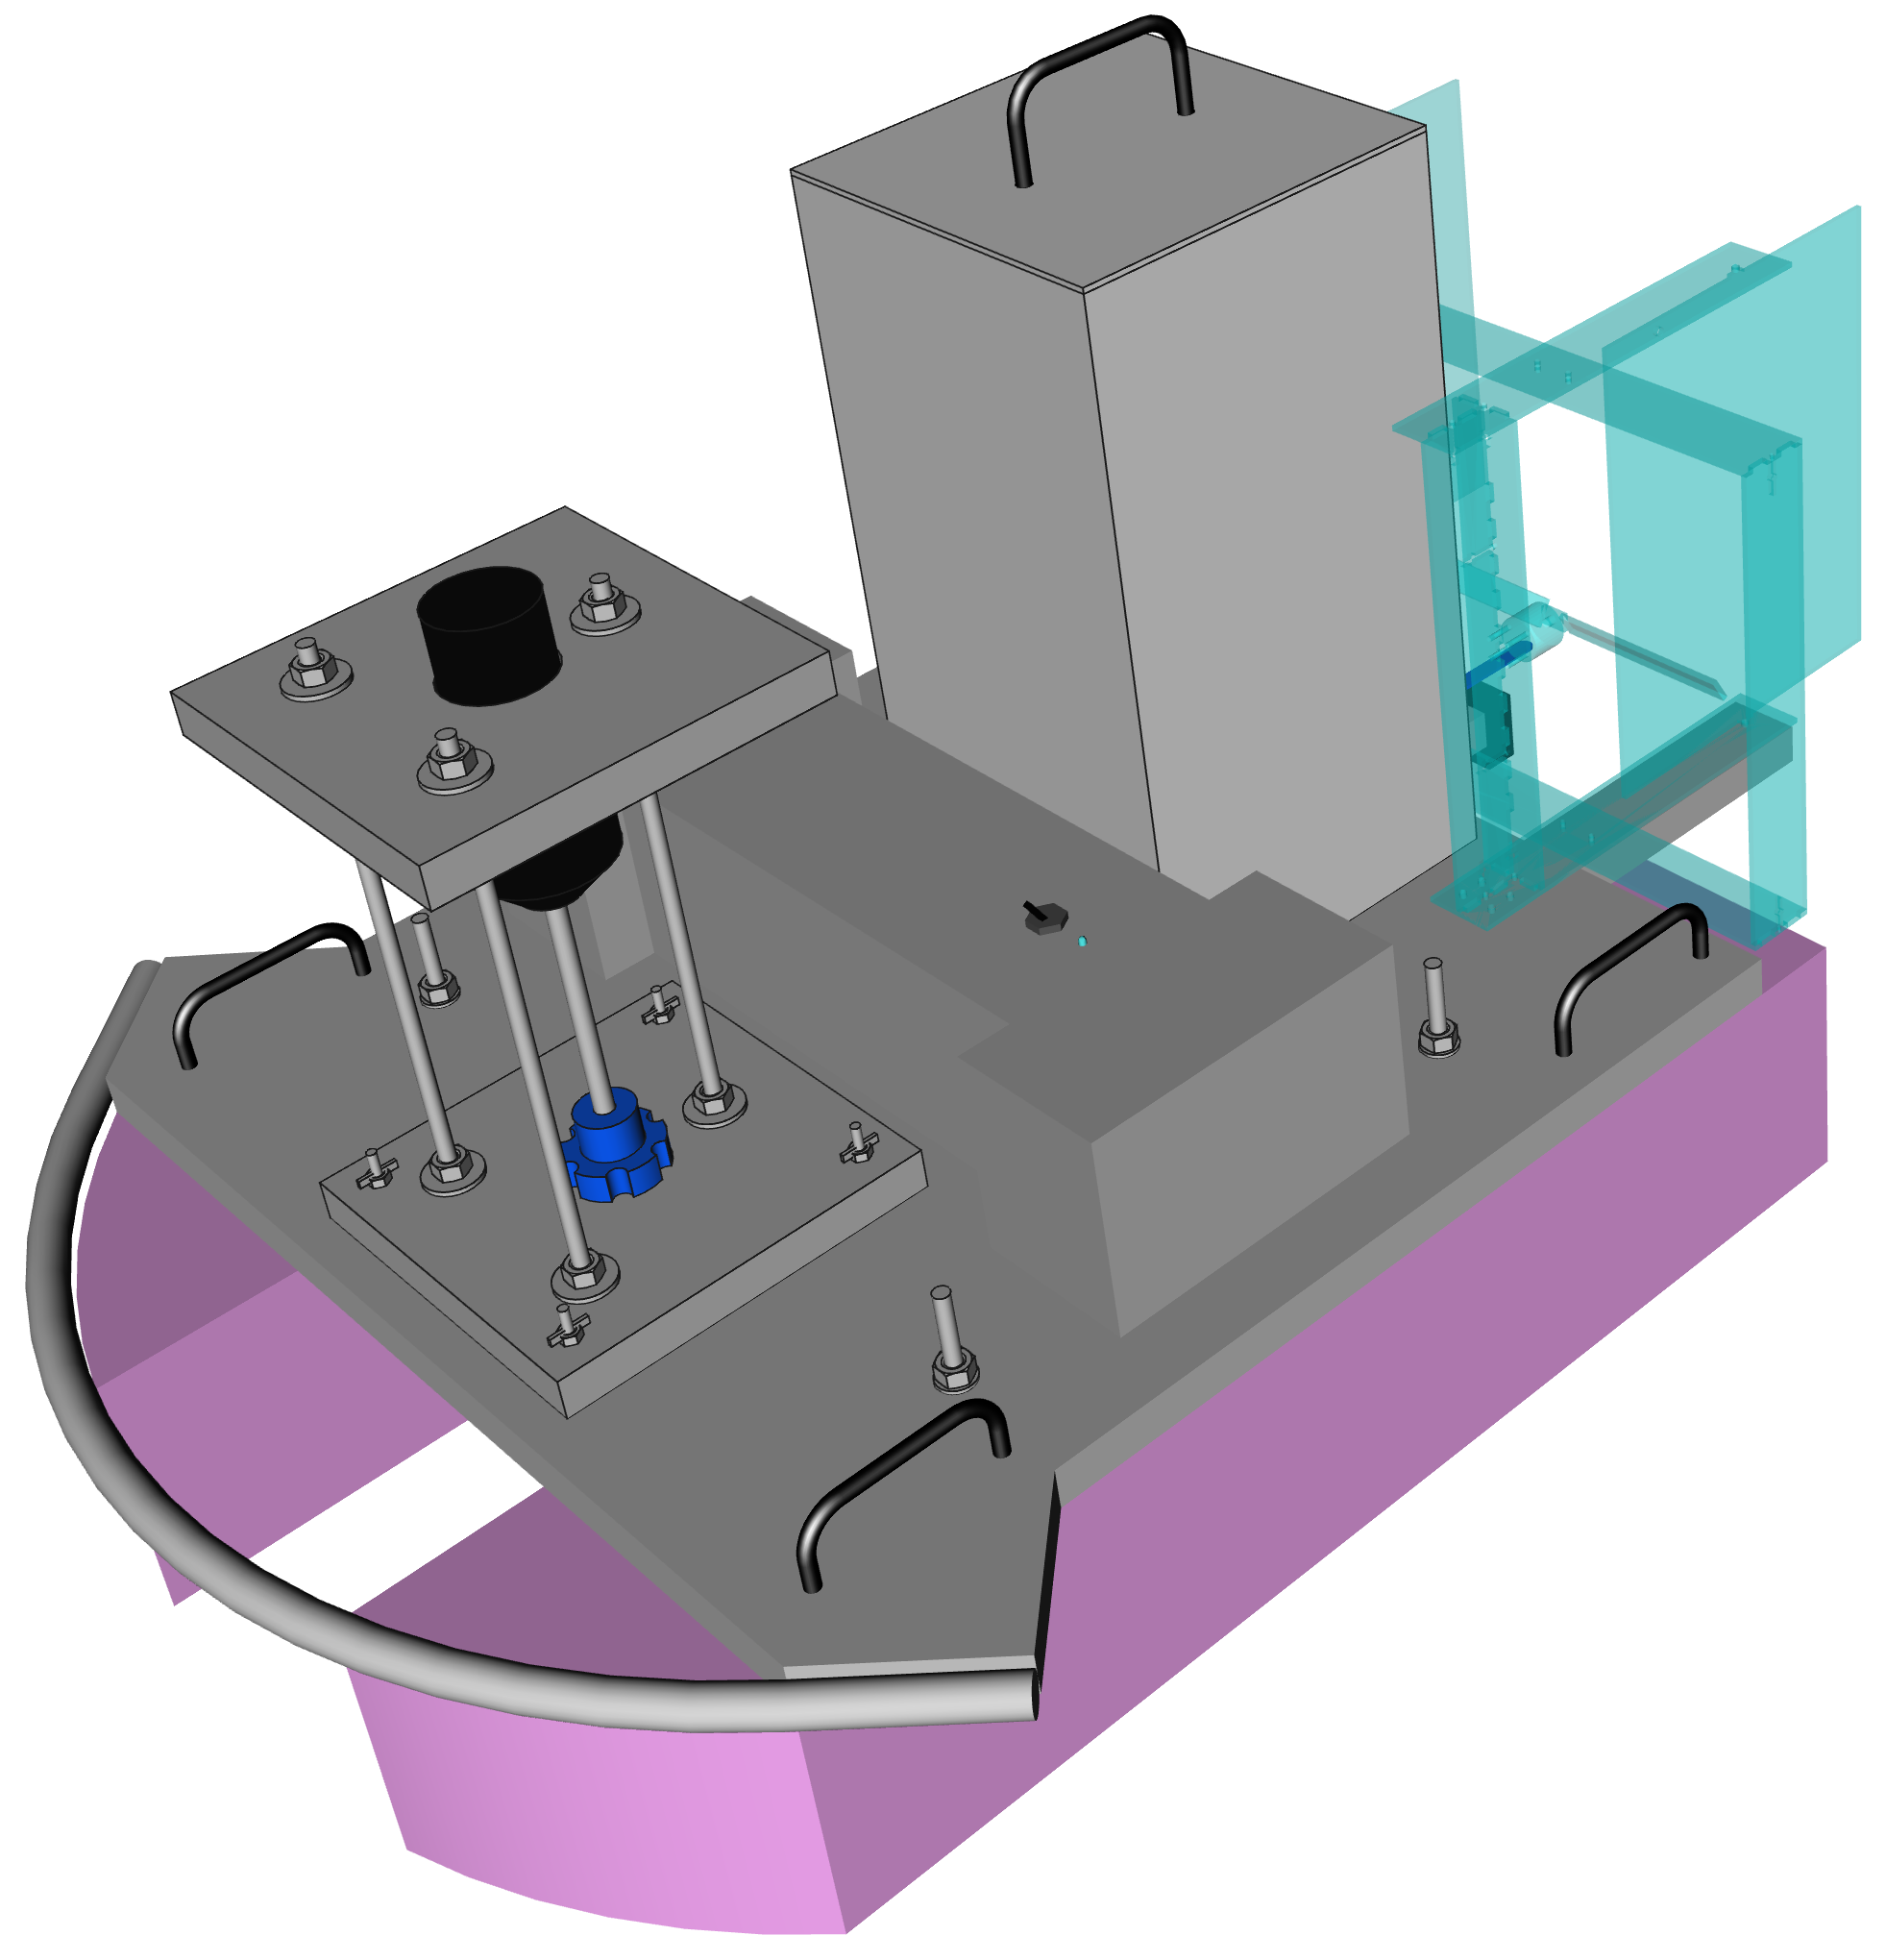
\includegraphics[width=27cm]{figures/front_box_off.png}}
        \end{figure}

      \end{block}

    \end{column}
    \begin{column}{\onecolwid}

      \begin{block}{Färdig prototyp}
        Den färdiga prototypen är billig att tillverka och använder till stor del
        färdiga komponenter. Byggmaterialet är utvalt för att vara återvinningsbart
        och lätt att arbeta med.

        På grund av framdrivning med luftpropellrar och roder uppnås god manöverbarhet
        även vid låga hastigheter.

        Batterikapaciteten är tillräcklig för att driva farkosten i mer än 60 minuter.

        \vskip 2cm
        \begin{figure}[H]
          \centering
          \hbox{\hspace{-3cm}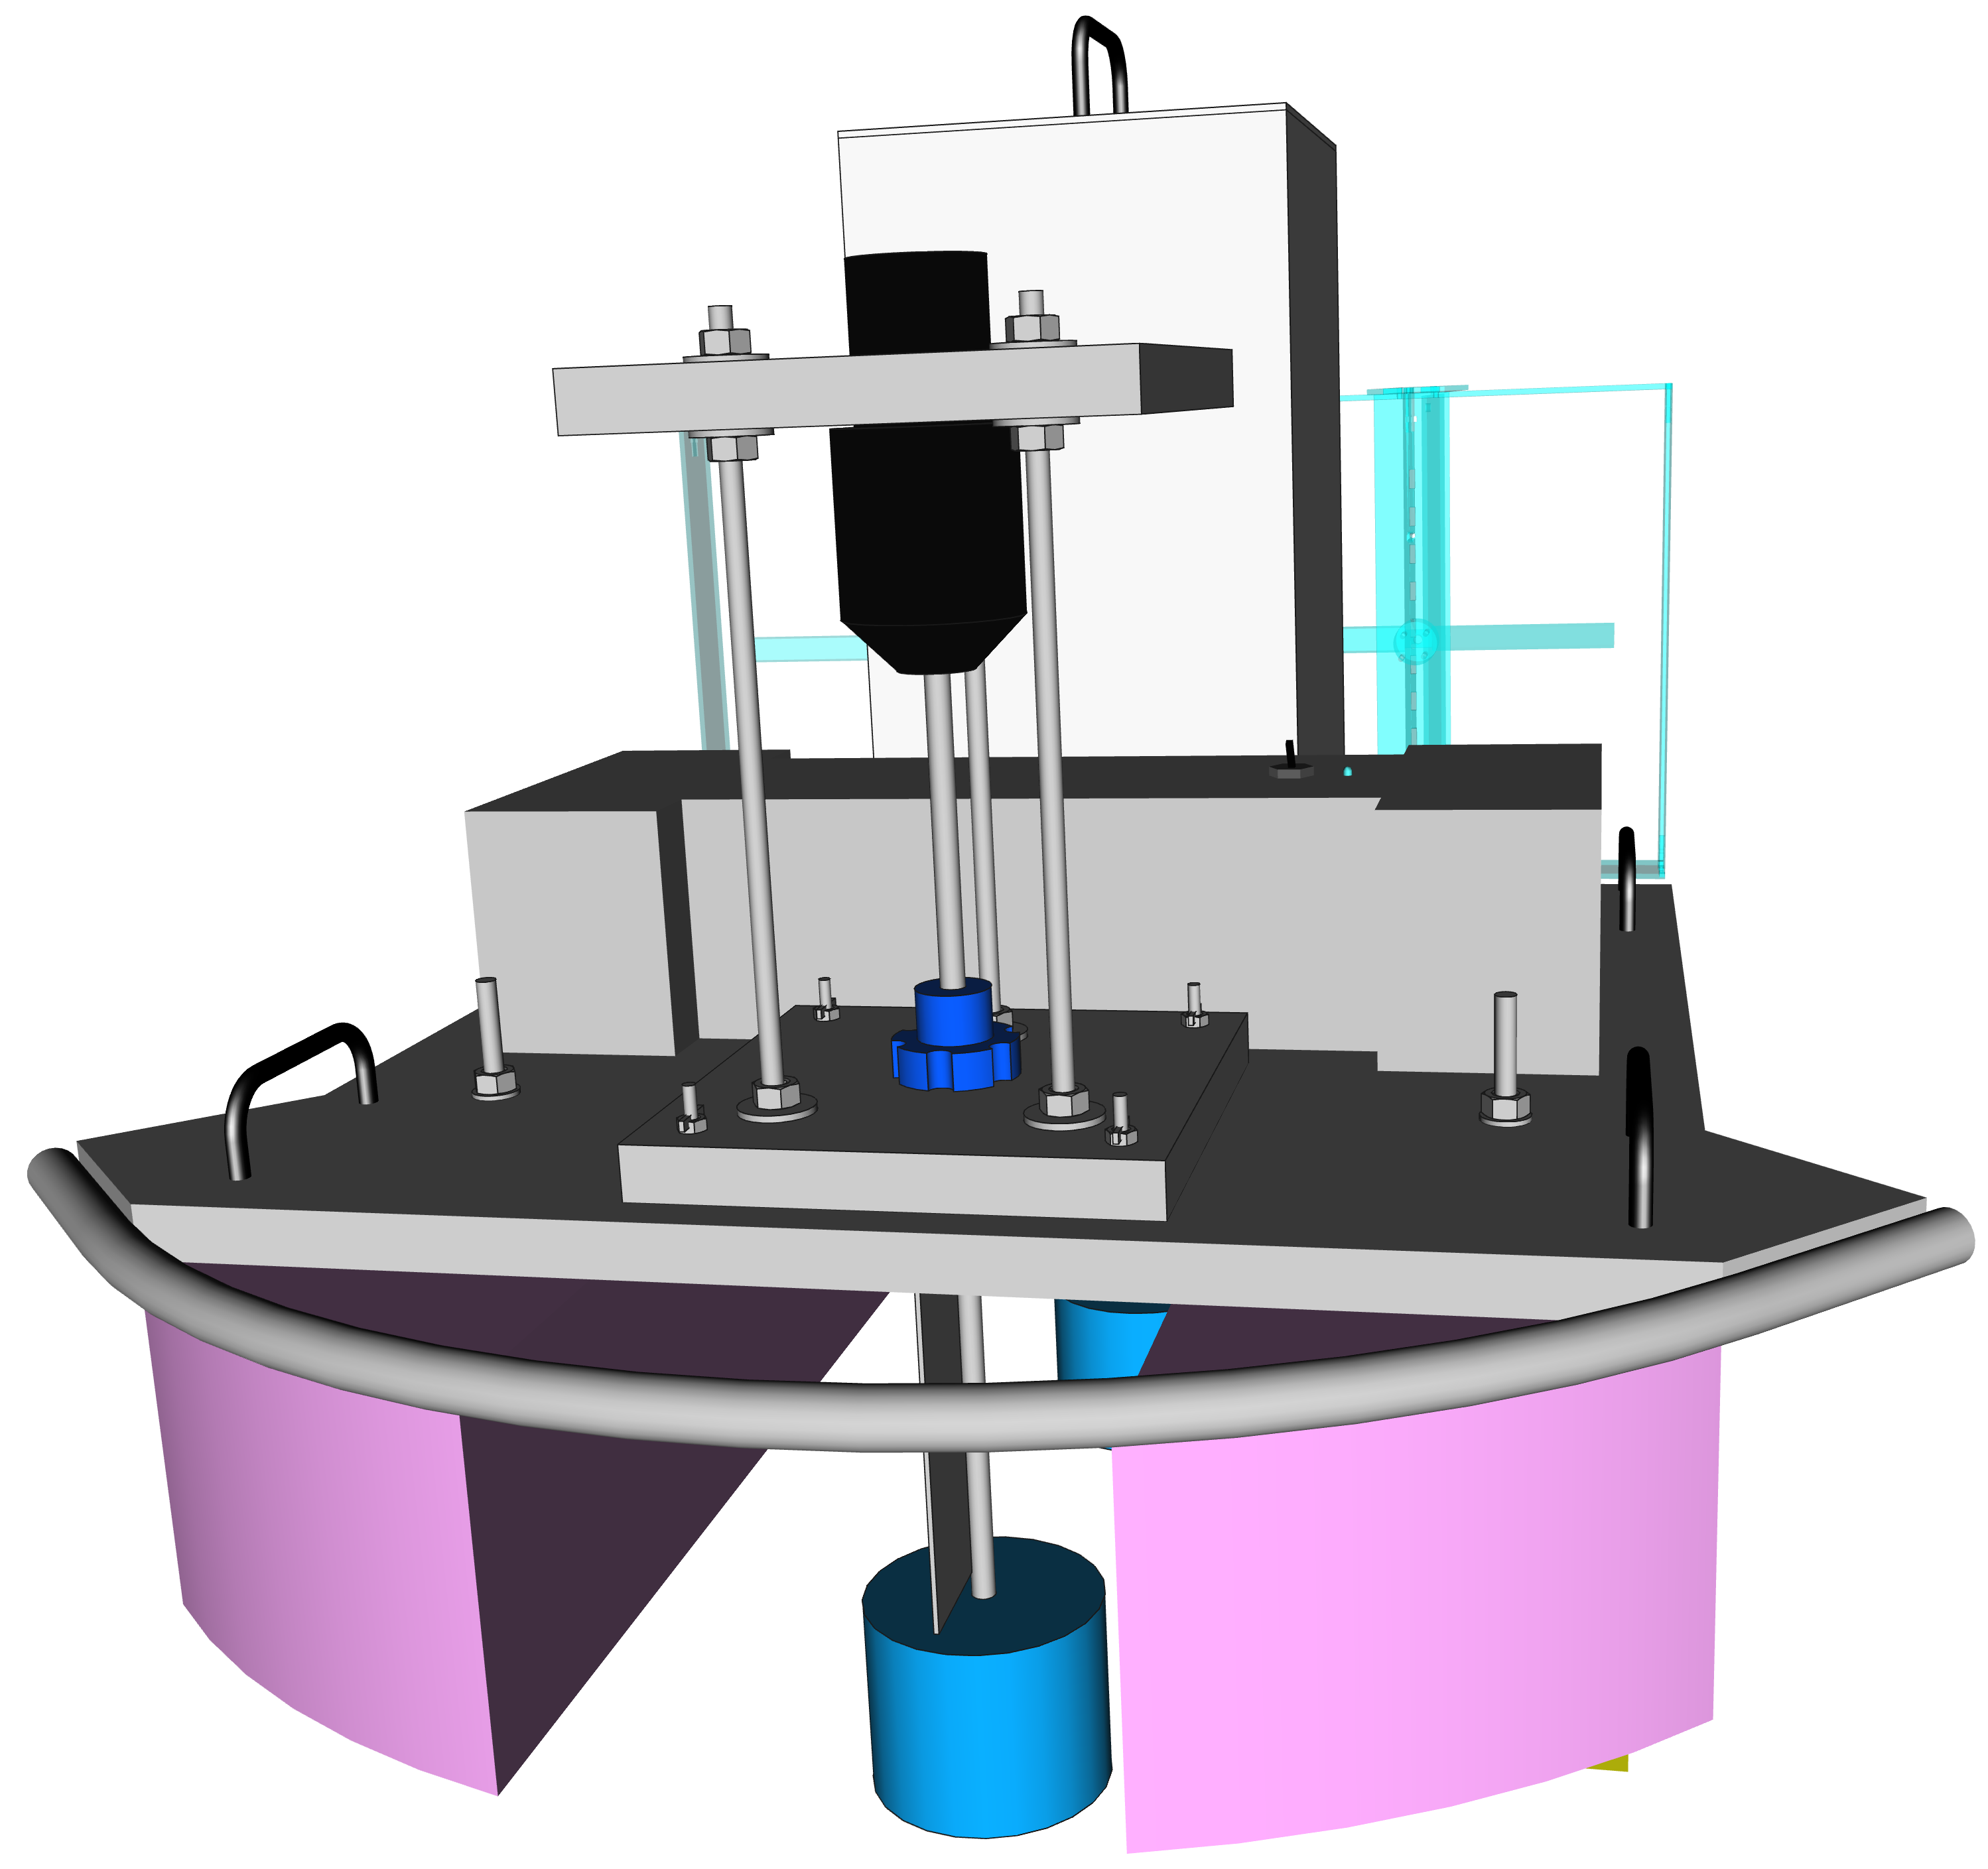
\includegraphics[width=25cm]{figures/front_rbr.png}}
        \end{figure}
      \end{block}

    \end{column}
    \begin{column}{\onecolwid}

      \begin{block}{Testresultat}
        \begin{itemize}
        \item I tester kunde flotten rena 2~m$^3$ av vår testlösning på ca 10 minuter.
        \item Bättre effekt än lokal stationär rening i samma vattenmassa.
        \end{itemize}

        \vskip 2cm
        \begin{figure}[H]
          \centering
          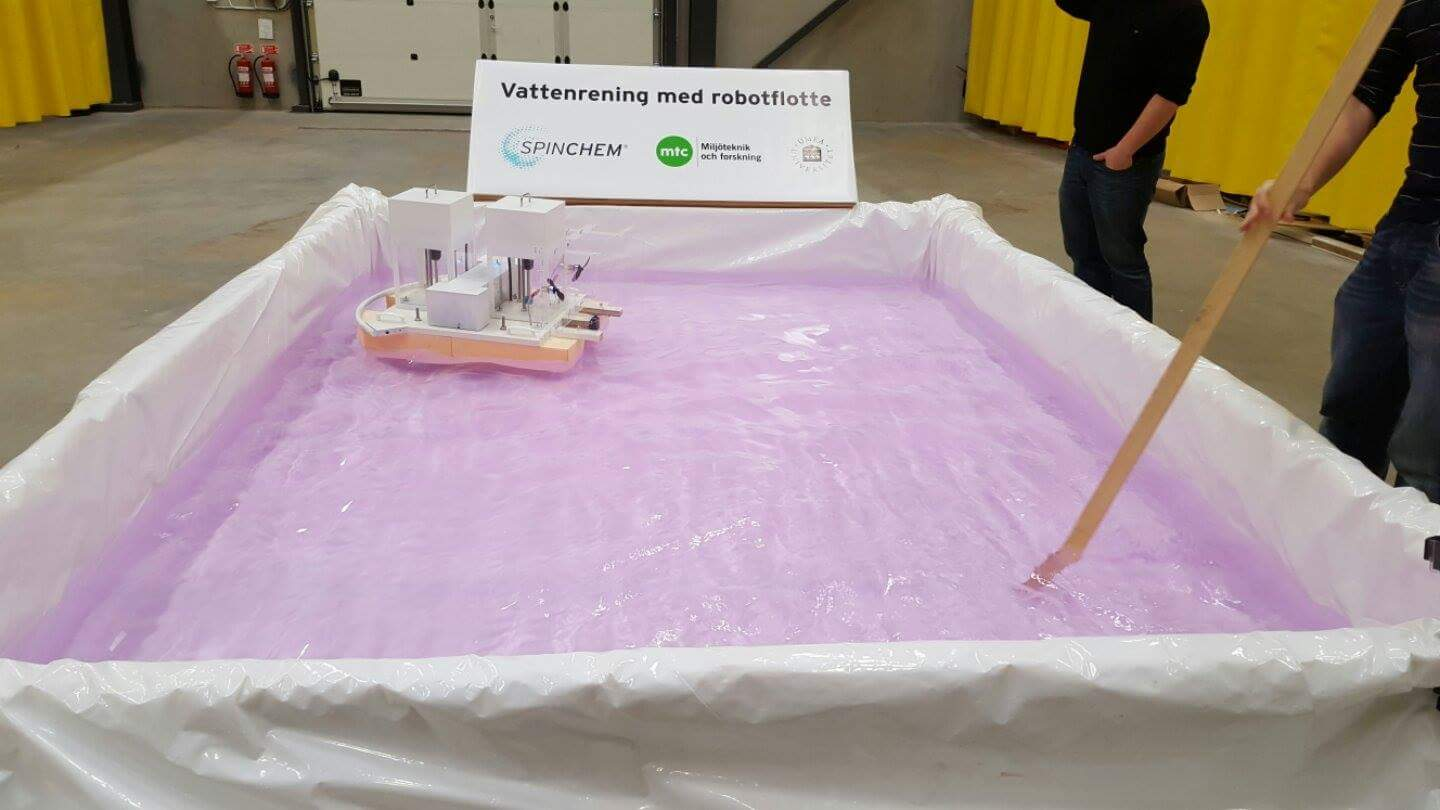
\includegraphics[width=\linewidth]{figures/pool.jpeg}
          \caption{Test i bassäng på Miljötekniskt Center i Umeå.}
        \end{figure}

        \vskip 2cm
        \begin{figure}[H]
          \centering
          \reflectbox{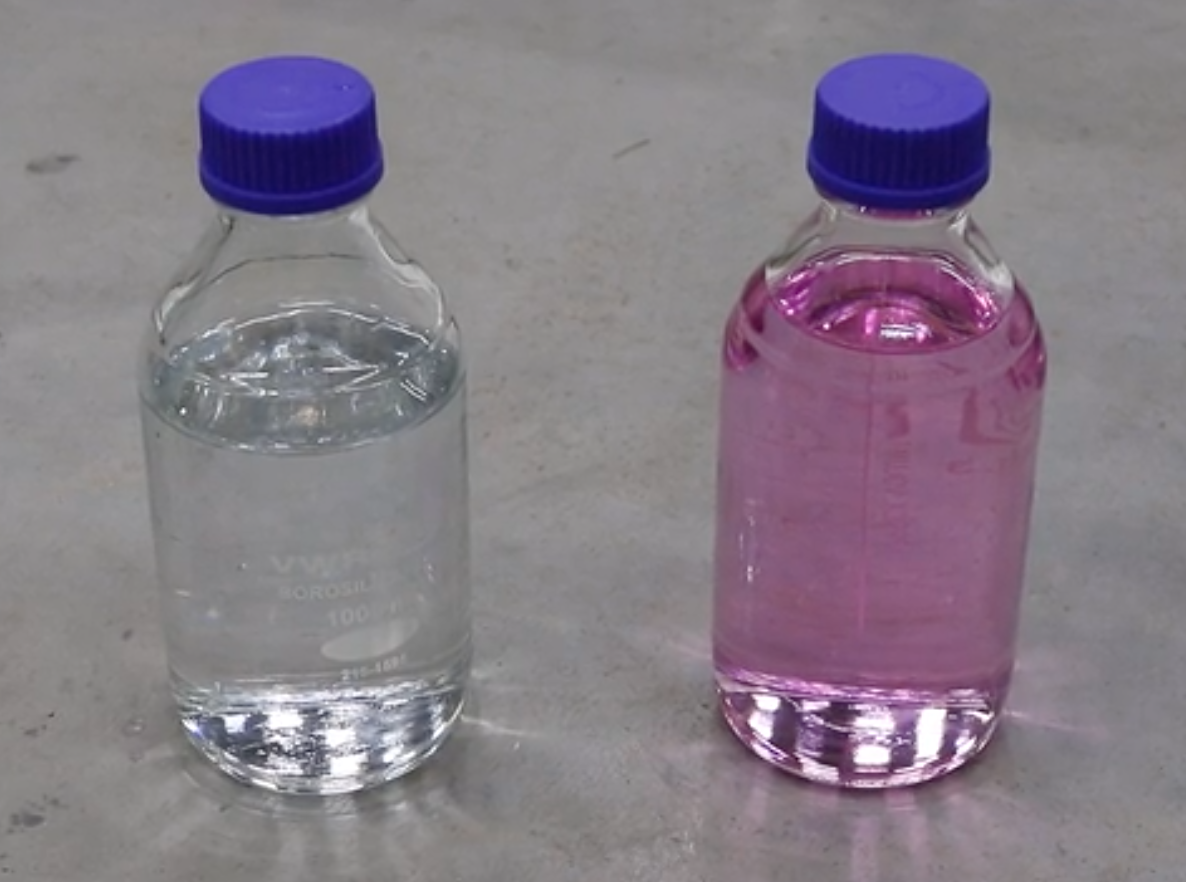
\includegraphics[width=\linewidth]{figures/samples.png}}
          \caption{Före- och efterprover.}
        \end{figure}

      \end{block}

    \end{column}

  \end{columns} % End of all the columns in the poster

\end{frame} % End of the enclosing frame

\end{document}
